\documentclass[a4paper,11pt]{article} 
\usepackage{tikz}
\usepackage{listings}
\usepackage[utf8]{inputenc}

\title{Artificial Intelligence Methods, exercise 3}
\author{Rendell Cale}
\date{\today}

\begin{document}

\maketitle

\paragraph{Implementing and testing decision-tree-learning}
I implemented the decision-tree-learning algorithm in python, trained it and ran on the test data. The final tree turned out to have $31$ nodes (when counting leaves which are decisions). 
A visualization of the tree is given below.


\resizebox{\linewidth}{150.0\lineheight}{
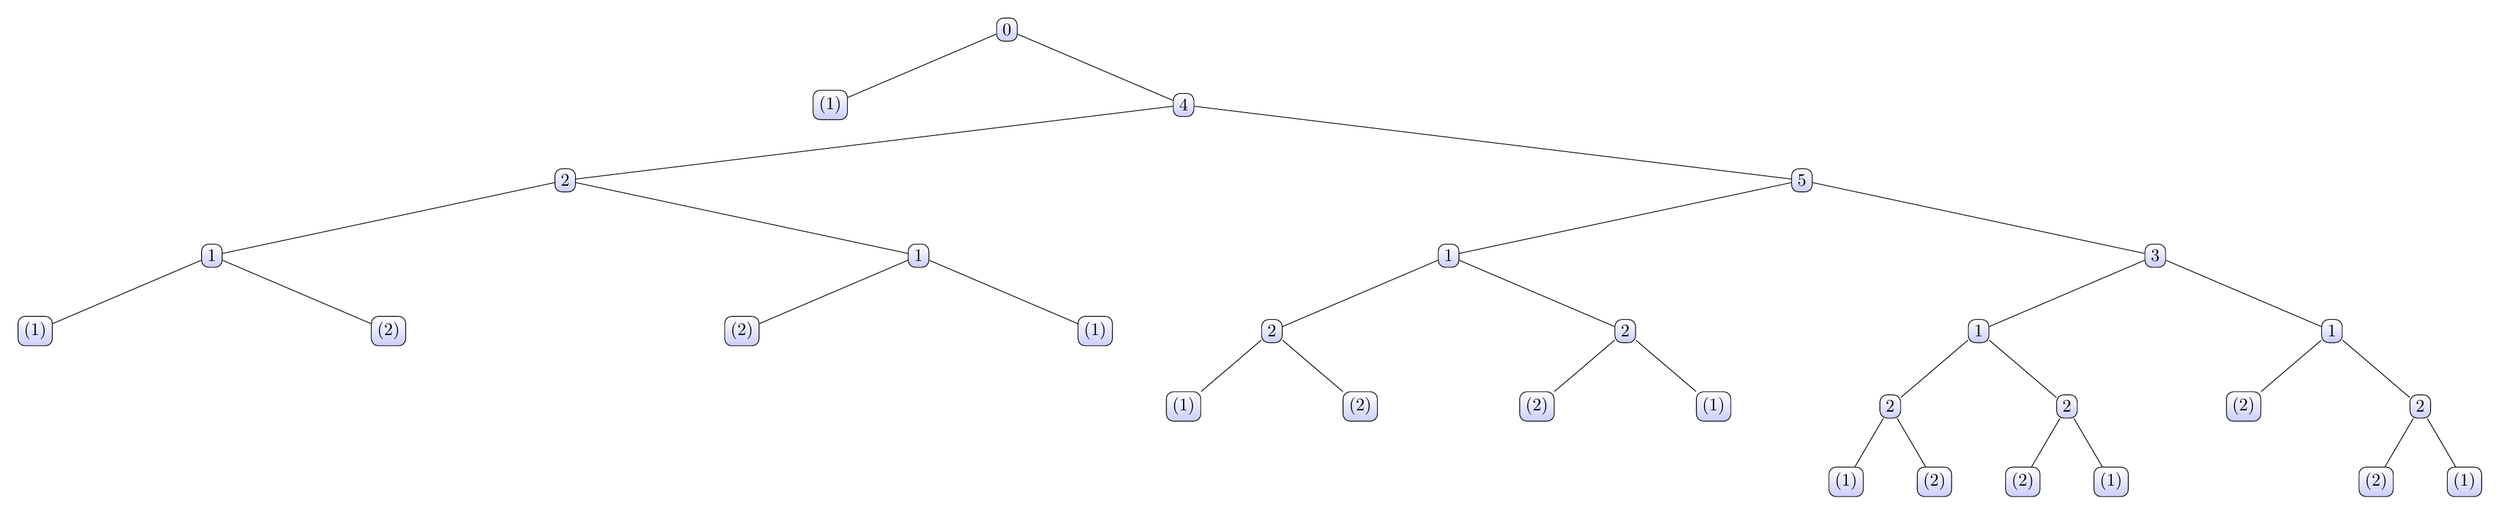
\begin{tikzpicture}[every node/.style = {shape=rectangle, rounded corners,
		draw, align=center, top color=white, bottom color=blue!20},
level 1/.style={sibling distance=20em},
level 2/.style={sibling distance=70em},
level 3/.style={sibling distance=40em},
level 4/.style={sibling distance=20em},
level 5/.style={sibling distance=10em},
level 6/.style={sibling distance=5em}]
	\node {0}child { node {(1)} } child { node {4}  child { node {2}   child { node {1}child { node {(1)} }child { node {(2)} }}   child { node {1}child { node {(2)} }child { node {(1)} }}}  child { node {5}   child { node {1}    child { node {2}child { node {(1)} }child { node {(2)} }}    child { node {2}child { node {(2)} }child { node {(1)} }}}   child { node {3}    child { node {1}     child { node {2}child { node {(1)} }child { node {(2)} }}     child { node {2}child { node {(2)} }child { node {(1)} }}}    child { node {1}child { node {(2)} }     child { node {2}child { node {(2)} }child { node {(1)} }}}}}};
\end{tikzpicture}
}




The internal node numbers indicate what attribute one should look at. If the attribute is $1$, go to the left subtree and if it is $2$ go to the right subtree. 

Testing it on the test data gave an accuracy of $92 \%$, and we get the same when we build the tree multiple times. It doesn't necessarily have to yield the same tree though, since the pluralityValue function uses randomness to break ties. 

When we build the tree with the random importance function, the trees change each time and have wildly different accuracies. I ran the algorithm and tested it ten thousand times to gather statistics on the performance and got the following results.

\lstinputlisting[language=bash]{ex3_results.txt}

From the results above we see that the information gain based approach has alot better performance on average than the random importance. By performance I mean mainly that the average tree size is smaller (31 vs 275) since both actually get same accuracy on average, $78 \%$. Note however that the random based approach got between $100 \%$ and $36 \%$, which is a big spread. Accuracy of $36 \%$ means that the decision tree is wrong more than right. Since there are only two alternatives it would then be better to do the opposite!

\paragraph{Conclusion}
Information gain importance is in better in that it is more consistent and tends to produce trees which are several orders of magnitude smaller. Since it uses the data to build to structure of the tree, it will probably also contain more information about the structure of the data. 

\end{document}

